\section{Sistema reale}
Dopo tutta l'introduzione teorica ed i calcoli mostrati, l'obiettivo di questo capitolo riguarderà la presentazione del sistema reale, la sua struttura, compresa di configurazione e le operazioni che hanno consentito la movimentazione.
\subsection{Struttura del robot}
Il manipolatore PKM è un manipolatore a cinematica parallela, composto da due braccia ed un end-effector. Alle braccia sono collegati due motori, uno per il braccio sinistro e l'altro per il braccio destro. Anche l'end-effector è composto da due motori, il primo motore permette di far salire/scendere la vite, il secondo invece genera un moto elicoidale che permette la rotazione della vite con conseguente salita/discesa. Un'altra parte fondamentale.
Per quanto riguarda la parte elettronica abbiamo la presenza di due azionamenti che sono collegati alle braccia e alla vite ed un modulo beckhoff che si occupa della gestione degli input digitali.
\subsubsection{Azionamenti}
Gli azionamenti utilizzati sono gli accelnet plus a 2 assi BE2, sono progettati appositamente per EtherCAT, operano con tensioni da 14 a 90 volt, riescono a fornire in uscita fino a 30A.
\\Sono predisposti per controllo in posizione, velocità e coppia di motori brushless, per la configurazione utilizzano il software CME 2 e la comunicazione avviene mediante l'interfaccia seriale RS-232. Il BE2 opera come ethercat slave, utilizzando il layer applicativo CAN su ethercat CoE. Inoltre, viene fornito un input AuxHV che permette in casi critici di tener vivo l'azionamento anche quando non c'è alimentazione senza perdere le informazioni sulla posizione o le comunicazioni con il sistema di controllo.
Per la comunicazione con ethercat invece sono predisposti due cavi RJ-45, la porta d'ingresso IN permette la connessione ad un master o alla porta d'uscita OUT di un dispositivo che nella gerarchia è interposto tra il master e l'azionamento. Inoltre, se l'accelnet è l'ultimo nodo della rete nonvi è bisogno di un terminatore sulla porta d'uscita.
 
\subsubsection{Beckhoff EK1814}
Il beckhoff EK1814 è un accoppiatore EtherCAT che fa da \textit{link} tra il protocollo EtherCAT a livello di bus di campo e il terminali EtherCAT. Inoltre, su questo modello sono anche integrati quattro input digitali e quattro output digitali. La sua struttura lo rende ideale per applicazioni con pochi input/output. L'accoppiatore converte i telegrammi che passano da Ethernet \textit{100BASE-TX} a rappresentazioni di segnali \textit{E-bus}. Una stazione EtherCAT è formata da un accoppiatore e da un numero N di terminali che vengono identificati automaticamente.
\\Inoltre, l'EK1814 ha due connessioni RJ45, l'interfaccia Ethernet superiore è utilizzata per collegare l'accoppiatore alla rete, mentre quella posteriore serve per il collegamento di altri dispositivi EtherCAT nello stesso commento. Nel nostro progetto è stato usato come master, a questo sono stati connessi gli slave (ovvero gli azionamenti), inoltre gli input e output digitali sono stati usati per controllare la pressione del fungo di emergenza e le luci di segnalazione delle fasi del manipolatore.
\subsubsection{Configurazione della rete}
La configurazione della rete prevede alla base della rete il PC Target, in questo vi è una chiavetta USB che permette di eseguire simulink real time. Il target ha due uscite ethernet, la prima è collegata direttamente al bechkoff, il quale prende l'identità di master, e come abbiamo visto precedentemente, al bechkoff sono attaccati e i due azionamenti che si comportano come slave.
\begin{figure}[ht]
\begin{center}
    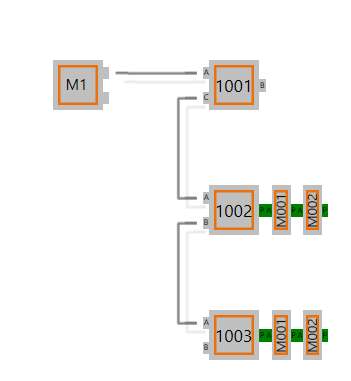
\includegraphics[scale=0.7]{Immagini/Sperimentale/network topology.PNG}
    \caption{Topologia della rete}
\end{center}
\end{figure}
Invece, alla seconda porta ethernet, vi è collegato il PC dell'utente, che provvede a generare, compilare, caricare ed eseguire i programmi sul PC target. Da User-PC è anche possibile vedere i grafici e fare delle analisi sui movimenti e le traiettorie eseguite dal manipolatore. La connessione avviene tramite una rete ethernet, l'indirizzo del target è 192.168.4.200, invece per User-PC:
\begin{figure}[ht]
\begin{center}
    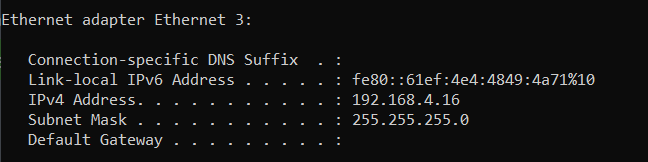
\includegraphics[scale=0.7]{Immagini/Sperimentale/ConfEthernet.png}
    \caption{Configurazione rete ethernet user PC}
\end{center}
\end{figure}
Dopo che è stata configurata la rete, sono stati configurati anche i messaggi, come è stato anticipato nella sezione precedente il metodo di comunicazione utilizzato è stato quello delle PDO. 
\begin{figure}[!ht]
\begin{subfigure}{.5\textwidth}
  \centering
  % include first image
  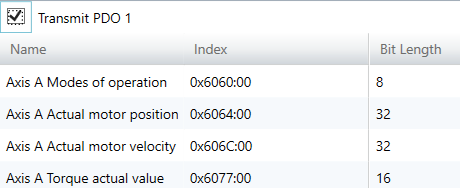
\includegraphics[width=.8\linewidth]{Immagini/Sperimentale/pdo1in.png}  
  \caption{PDO Input 1}
  \label{fig:sub-firstpdo}
\end{subfigure}
\begin{subfigure}{.5\textwidth}
  \centering
  % include second image
  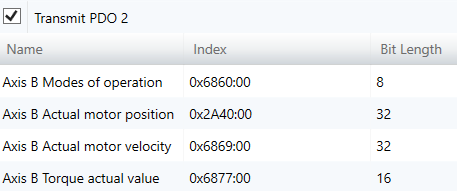
\includegraphics[width=.8\linewidth]{Immagini/Sperimentale/pdo2in.png}  
  \caption{PDO Input 2}
  \label{fig:sub-secondpdo}
\end{subfigure}
\begin{subfigure}{.5\textwidth}
  \centering
  % include third image
  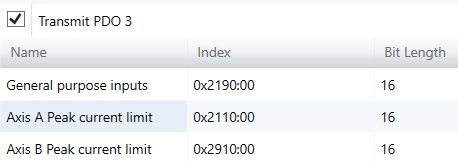
\includegraphics[width=.8\linewidth]{Immagini/Sperimentale/pdo3in.png}  
  \caption{PDO Input 3}
  \label{fig:sub-thirdpdo}
\end{subfigure}
\begin{subfigure}{.5\textwidth}
  \centering
  % include fourth image
  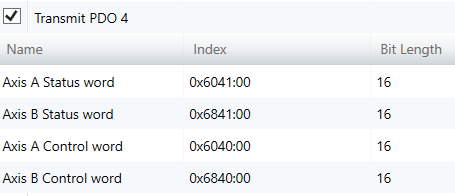
\includegraphics[width=.8\linewidth]{Immagini/Sperimentale/pdo4in.png}  
  \caption{PDO Input 4}
  \label{fig:sub-fourthpdo}
\end{subfigure}
\caption{PDO in input}
\end{figure}
\begin{figure}[ht]
\begin{center}
    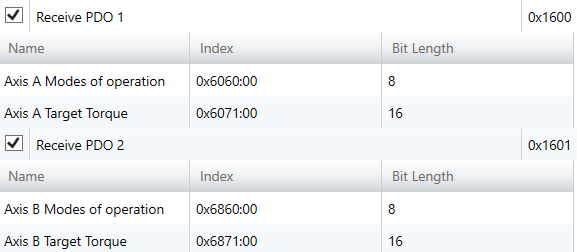
\includegraphics[scale=0.7]{Immagini/Sperimentale/pdo12out.png}
    \caption{PDO Output 1 e 2}
\end{center}
\end{figure}
Nelle immagini appena presentate vi sono i parametri che vengono trasmessi mediante le PDO, sono tutti parametri che servono per far operazioni di movimentazione e di controllo, più avanti verranno analizzati nel particolare.
\subsection{Stateflow}
\textit{Stateflow} si occupa di fornire diagrammi di transizione, stato e di flusso utilizzando un linguaggio grafico. Nel caso del manipolatore è stato utilizzato per la progettazione di diagrammi di transizione in base agli stati del robot. In questa sezione andremo a vedere le fasi gli stadi di evoluzione che sono stati costruiti.
\subsubsection{Fase di Homing}
Il primo stadio è quello di \textit{homing}, consiste nel portare allo "zero" i motori, quindi quelo delle braccia e quello della vite. Per zero si intende portarli a toccare il finecorsa ed indicargli che quello è il loro punto di partenza.
\begin{figure}[ht]
\begin{center}
    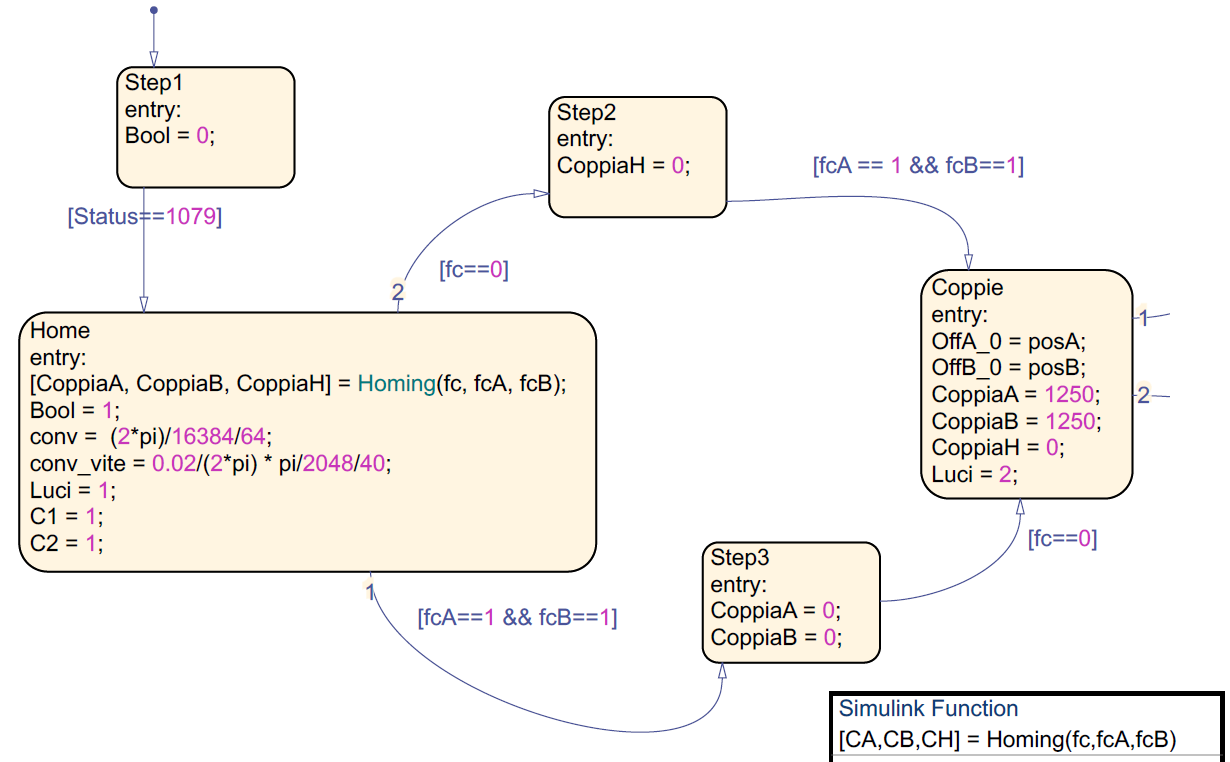
\includegraphics[scale=0.55]{Immagini/Sperimentale/state1.png}
    \caption{State flow: fase di homing}
\end{center}
\end{figure}
Passiamo nel primo stato, quando la \textit{Status Word} è uguale a 1079, ovvero quando gli azionamenti sono usciti dalla fase \textit{pre-operational}. Non appena entriamo nello stato successivo, identificato dal nome \textbf{Home}, viene eseguita una funzione matlab che si occupa di dare le coppie sufficienti alla movimentazione ai motori di entrambe le braccia e ad uno dei motori della vite, in particolare al motore che permette la traslazione per l'asse Z ma non la rotazione. Una volta raggiunta la posizione del finecorsa le coppie vengono settate a 0, impedendo quindi un'ulteriore movimentazione. 
\subsubsection{Fase di posizionamento}
La fase successiva è quella di posizionamento, per semplicità infatti si è scelto di mettere il robot in una configurazione predefinita e non lasciarlo in finecorsa per quanto riguarda le braccia, mentre per quanto riguarda la vita si è scelto di far abbassare la vite di una quantità predefinita per farle toccare un foglio e di conseguenza per predisporla al disegno. Le angolazioni scelte per il robot sono state $80^\circ$ e $100^\circ$, partendo da $-30^\circ$ e $60^\circ$
\begin{figure}[ht]
\begin{center}
    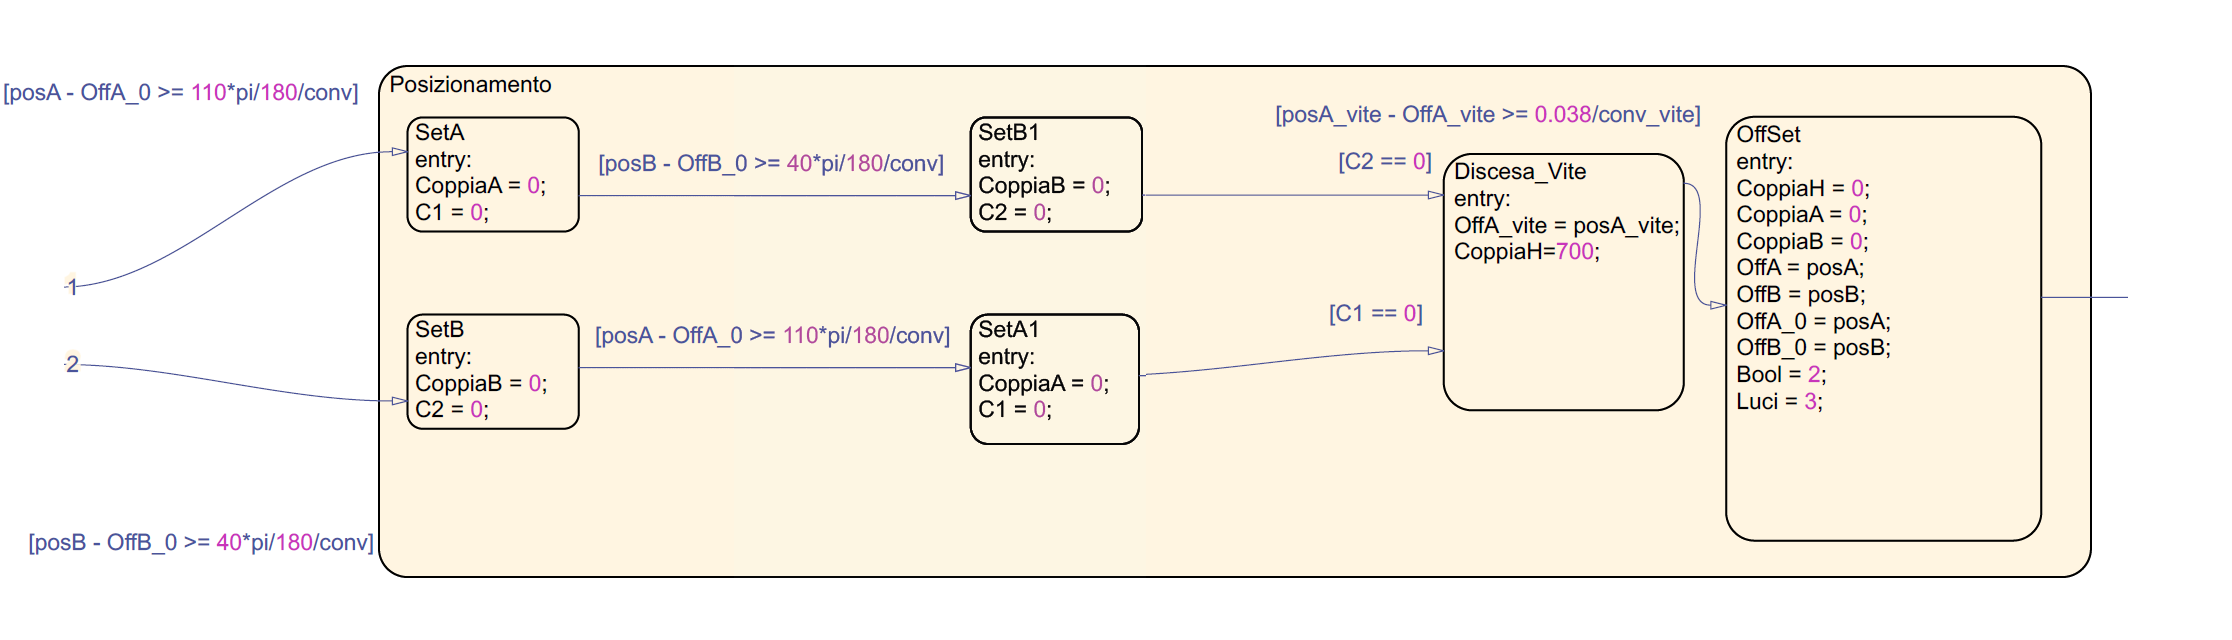
\includegraphics[scale=0.31]{Immagini/Sperimentale/state2.png}
    \caption{State flow: fase di posizionamento}
\end{center}
\end{figure}
Come si può vedere dallo schema in figura viene prima eseguita la movimentazione delle braccia, per l'asse A di $40^\circ = 100^\circ - 60^\circ$ e per l'asse B di $110^\circ = 80^\circ + 30^\circ$, successivamente viene fatta scendere la vite di 38mm. Dopo che la vite si è posizionata vengono settati gli \textit{offset} di posizione, questo serve in quanto i motori si muovono aumentando il valore dei \textit{counts}, settando però un'\textit{offset} possiamo essere sicuri di aver una scala temporale corretta.
\subsubsection{Fase di traiettoria}
L'ultima fase è quella della traiettoria, in questa fase ri-settiamo gli offset della vite in quanto il posizionamento è stato appena concluso ed andiamo a settare l'offset del tempo, questo ci permette di far partire virtualmente il tempo da zero dopo che è stata raggiunta la configurazione finale di \textit{homing}. 
\begin{figure}[ht]
\begin{center}
    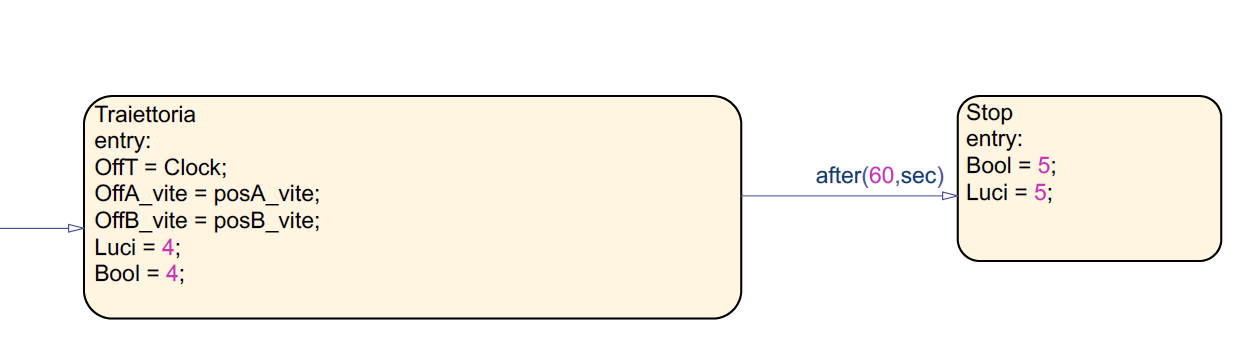
\includegraphics[scale=0.55]{Immagini/Sperimentale/state3.png}
    \caption{State flow: traiettoria}
\end{center}
\end{figure}
Durante tutte le fasi anche due variabili si evolvono costantemente, queste sono bool e luci, la prima ci va ad indicare lo stato preciso in cui ci troviamo in base alla seguente tabella:
\begin{table}[h!]
\centering
\begin{tabular}{|c |c |} 
 \hline
 Valore & Stato \\ [0.5ex] 
 \hline\hline
  0  & pre-operazionale \\ 
  1 & Homing \\
  2 & Manipolatore posizionato\\
  3 & Traiettoria\\
  4 & Manipolatore fermo\\
 \hline
\end{tabular}
\caption{Valori di \textit{bool}}
\label{table:3}
\end{table}
la seconda invece serve a pilotare le luci in modo che si ha un feedback visuale della fase in cui è il manipolatore.
\begin{table}[h!]
\centering
\begin{tabular}{|c |c|c|} 
 \hline
 Valore & Colore & Bool \\ [0.5ex] 
 \hline\hline
  1  & Bianco & 1 \\ 
  2 &  Bianco Rosso & 1\\
  3 &  Rosso & 2 \\
  4 & Bianco Verde & 3\\
  5 & Verde & 4\\
 \hline
\end{tabular}
\caption{Valori delle luci}
\label{table:4}
\end{table}
Dopo che il manipolatore entra nello stato della traiettoria quest'ultima viene eseguita in base ad una selezione, per passare allo stato successivo invece dovranno passare 60 secondi, l'ultimo stato è uno stato di fermo, il manipolatore ha finito la traiettoria e di conseguenza va in "riposo" mettendo a zero tutte le coppie.
\subsection{Struttura del manipolatore}
\subsubsection{Sistema vite}
\subsubsection{Sistema braccia}
\subsubsection{Gestione della traiettoria}
\subsection{Controllo}
In questa sezione andremo a vedere le tipologie di controllo che sono state utilizzate, verranno mostrati anche dei grafici e delle analisi relative a questi metodi.
\subsubsection{Controllo Vite}
\subsubsection{Controllo PD}
\subsubsection{Controllo in dinamica inversa}
Il primo controllo per il robot è stato fatto mediante l'utilizzo di un proporzionale che comprendeva la somma di posizione e velocità, si è riscontrato che a causa del mancato contributo derivativo ed integrativo la traiettoria non veniva seguita in maniera del tutto corretta, ed alzano il valore di $K_p$ troppo le vibrazioni aumentavano, si è quindi cercato inizialmente di trovare un punto nel quale il manipolatore non vibrava e non oscillava. Successivamente si è andato ad applicare un controllo in dinamica inversa, la prima tipologia di controllo scelta è stata quella in anello aperto [inscerisci schema], dopo i test effettuati con questa tipologia di controllo si è riscontrato che le coppie risultati erano basse, all'incirca $0.5 C_m$, con $C_m$ la coppia per far muovere il manipolatore. L'approccio successivo è stato quello di continuare con la dinamica inversa ma chiudendo l'anello, [inserisci schema]
Un test che è stato fatto per andare a ricercare i parametri è stato quello di far variare $K_p$, in un range di valori compreso tra 350 e 950 ad intervalli di 50, in base ad un valore fisso di $K_d$, andiamo ora a vedere un risultato di questo metodo.
\begin{figure}[!ht]
\begin{subfigure}{.5\textwidth}
  \centering
  % include first image
  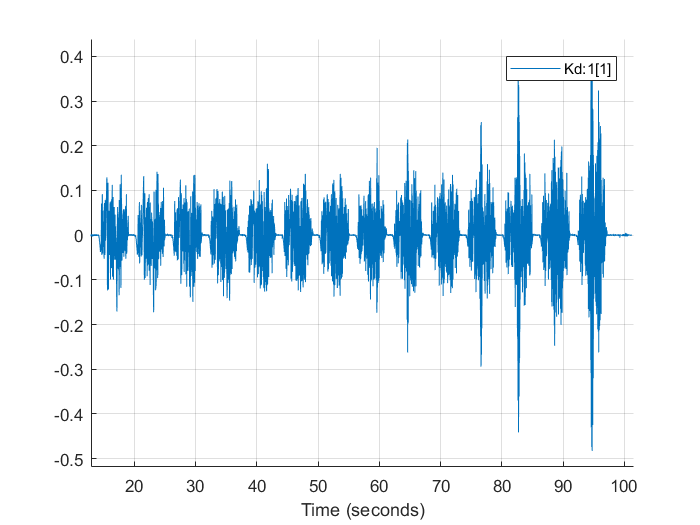
\includegraphics[width=.8\linewidth]{Immagini/Sperimentale/Test_Kd=1.5.png}  
  \caption{Test con $K_d$ = 1.5}
  \label{fig:sub-kd1.5}
\end{subfigure}
\begin{subfigure}{.5\textwidth}
  \centering
  % include second image
  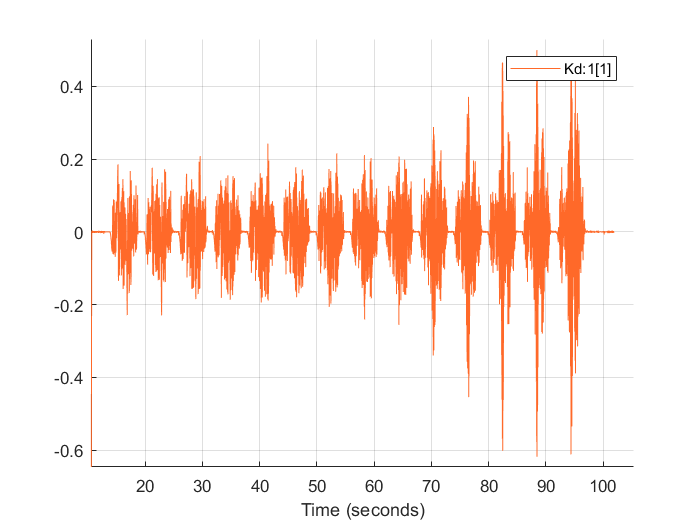
\includegraphics[width=.8\linewidth]{Immagini/Sperimentale/Test_Kd=2.png}  
  \caption{Test con $K_d$=2}
  \label{fig:sub-kd2}
\end{subfigure}
\begin{subfigure}{.5\textwidth}
  \centering
  % include third image
  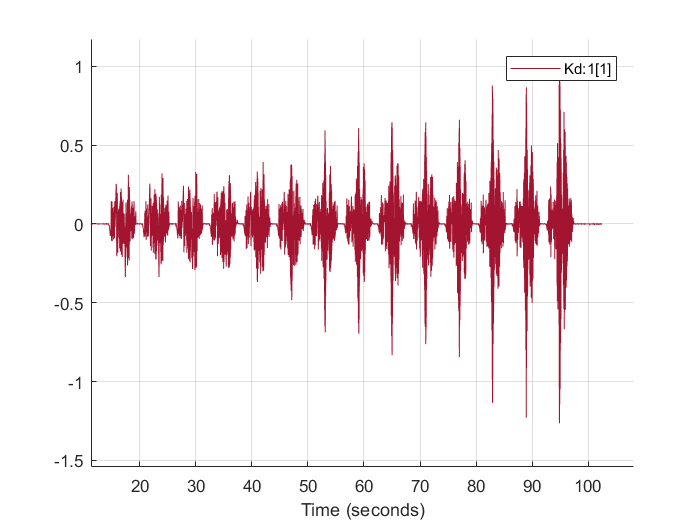
\includegraphics[width=.8\linewidth]{Immagini/Sperimentale/Test_Kd=3.png}  
  \caption{Test con $K_d$=3}
  \label{fig:sub-kd3}
\end{subfigure}
\begin{subfigure}{.5\textwidth}
  \centering
  % include third image
  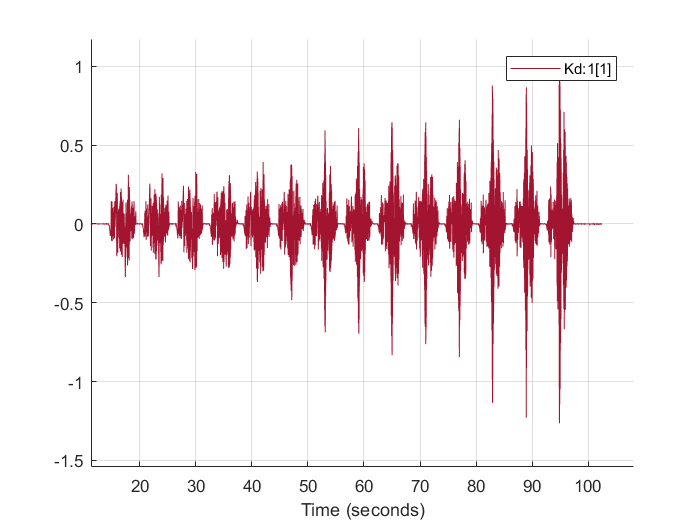
\includegraphics[width=.8\linewidth]{Immagini/Sperimentale/Test_Kd=3.png}  
  \caption{Test con $K_d$=3}
  \label{fig:sub-kd1}
\end{subfigure}
\caption{Test su $K_d$}
\end{figure}
Si può chiaramente vedere come all'aumentare di $K_d$ i valori di $K_p$ iniziano ad vibrare sempre prima. Come valori finali per questo controllore sono stati scelti $K_d = \frac{3}{2}$ e $K_p = 720$
\subsection{Traiettorie eseguite}
In questa sezione andremo a vedere ed analizzare tutte le traiettorie che sono state create, le traiettorie variano da bidimensionali a tridimensionali, andando anche ad includere due pattern.